\documentclass[12pt]{article}

% Package Imports
\usepackage{amsmath,amssymb}  % Math symbols
\usepackage{graphicx}         % For figures
\usepackage[margin=1in]{geometry}  % Standard margin
\usepackage{setspace}         % Adjust line spacing
\usepackage{authblk}          % For authors and affiliations
\usepackage{caption}          % For figure captions
\usepackage{subfigure} 
\usepackage[numbers, sort]{natbib} % 保证参考文献不会出现乱序

% Title and Author Setup
\title{quantms, ms2rescore and multiple search engines enables deep proteome coverage across protein quantification, immunopeptidomics, and phosphoproteomics experiments}
\author[1,2]{Dai Chengxin}
\author[3]{Ralf Gabriels}
\author[3]{Robbin Bouwmeester}
\author[4,5,6,7]{Jonas Scheid}
\author[8]{Mingze Bai}
\author[9,7]{Timo Sachsenberg}
\author[10]{Yasset Perez-Riverol\thanks{Corresponding author: yperez@ebi.ac.uk}}
\affil[1]{State Key Laboratory of Medical Proteomics, Beijing Proteome Research Center, National Center for Protein Sciences (Beijing), Beijing Institute of Lifeomics, 102206, Beijing, China}
\affil[2]{International Academy of Phronesis Medicine (Guangdong), 510320, Guangdong, China}
\affil[3]{VIB-UGent Center for Medical Biotechnology, VIB, 9052 Ghent, Belgium}
\affil[4]{Department of Peptide-based Immunotherapy, Institute of Immunology, University and University Hospital Tübingen, Tübingen, Germany}
\affil[5]{Cluster of Excellence iFIT (EXC2180) "Image-Guided and Functionally Instructed Tumor Therapies", University of Tübingen, Tübingen, Germany}
\affil[6]{Quantitative Biology Center (QBiC), University of Tübingen, Tübingen, Germany}
\affil[7]{Institute for Bioinformatics and Medical Informatics (IBMI), University of Tübingen, Tübingen, Germany}
\affil[8]{Chongqing Key Laboratory of Big Data for Bio Intelligence, Chongqing University of Posts and Telecommunications, Chongqing, China}
\affil[9]{Department of Computer Science, Applied Bioinformatics, University of Tübingen, Tübingen, Germany}
\affil[10]{European Molecular Biology Laboratory, European Bioinformatics Institute, Wellcome Genome Campus, Cambridge, United Kingdom}
\date{}

% Document Begins
\begin{document}
\maketitle
\doublespacing  % MCP requires double-spacing

% Abstract Section
\begin{abstract}
The exponential growth of public proteomics datasets has outpaced the capacity of traditional desktop tools for large-scale automated analysis. This study presents an integrated workflow combining quantms, a cloud-native pipeline, with MS2Rescore, a machine learning-driven rescoring tool, to enable deep reanalysis of massive proteomic datasets. Leveraging the Nextflow workflow engine for parallel computing, the pipeline integrates fragment ion intensity and retention time predictions from MS2PIP and DeepLC to optimize peptide-spectrum match reliability via Percolator. Across four benchmark datasets spanning label-free quantification, TMT labeling, immunopeptidomics, and phosphoproteomics, the workflow demonstrates a 16–22.8\% increase in identified spectra compared to traditional approaches, with hundreds of newly quantified proteins and phosphosites. The results highlight that multi-search-engine collaboration with machine learning-derived features not only enhances identification sensitivity but also deepens quantitative insights for downstream biological discoveries. This approach provides a reproducible solution for large-scale reanalysis of public proteomics data, aligning with FAIR principles for scientific accessibility and reuse.

\end{abstract}

% Keywords
\noindent\textbf{Keywords:} Proteomics, Reanalysis, Workflow, Machine learning.

% Main Content
\section{Introduction}
In recent years, the field of proteomics has experienced rapid growth in the availability of publicly accessible datasets, accompanied by a shift toward studies analyzing larger sample cohorts. As of June 2025, over 40,000 datasets have been submitted to ProteomeXchange (PX) repositories, including a substantial increase in large-scale submissions comprising more than 100 instrument files \cite{perez-riverol_pride_2025}. However, conventional desktop tools such as MaxQuant \cite{cox_maxquant_2008}, pFind \cite{wang_pfind_2007}, PeptideShaker \cite{vaudel2015peptideshaker}, and Proteome Discoverer are limited in their capacity to perform automated, large-scale quantitative analyses in cloud or distributed environments, hindering the reanalysis of extensive experiments on standard workstations.

We recently developed quantms \cite{dai_quantms_2024}, an open-source, cloud-based pipeline designed for massively parallel reanalysis of quantitative proteomic datasets. The pipeline is highly modular and flexible, accommodating a wide range of quantitative proteomics approaches including DDA label-free, DDA multiplex (TMT and ITRAQ) and DIA. quantms automatically distributes computations using the Nextflow workflow engine across one or more computing nodes, depending on the number of instrument files and samples \cite{di_tommaso_nextflow_2017}. To ensure traceability and reproducibility, the pipeline is built entirely on standardised open file formats and reproducible execution environments, adhering strictly to the FAIR (Findability, Accessibility, Interoperability, and Reusability) principles \cite{wilkinson_fair_2016}. quantms has been extensively benchmarked and used in the analysis of large-scale public proteomics datasets \cite{dai_quantms_2024,bai2023lfq, ZHENG2025105440}.

With the integration of machine learning (ML) into proteomics, various models have been developed to accurately predict peptide properties, such as MS2PIP \cite{degroeve_ms2pip_2013} for fragment ion intensities and DeepLC \cite{bouwmeester_deeplc_2021} for retention time prediction. Early approaches employed decision trees and single-layer neural networks, while more recent deep learning models such as Prosit \cite{gessulat_prosit_2019} achieve significantly improved accuracy for predicting fragment ion intensities and retention times. These highly accurate predictions enable superior matching of experimental data to theoretical expectations and have reinvigorated rescoring strategies in proteomics.

Previously, quantms did not leverage measurable peptide properties such as fragment ion intensities and retention times. To overcome this limitation, we integrated MS2Rescore into quantms and incorporated customized features following Nextflow and nf-core best practices. We demonstrate that the enhanced pipeline supports in-depth analysis of large-scale public proteomics datasets across diverse experimental designs, including LFQ, TMT, immunopeptidomics, and phosphoproteomics studies.

\section{Methods}

\subsection{MS/MS Data and quantms Search Results}
To develop and evaluate the performance of the quantms-integrated MS2Rescore workflow, four publicly available benchmark datasets were downloaded from PRIDE Archive under the identifiers PXD001819, PXD019643, and PXD026824, and from CPTAC under the identifier PDC000125. The PXD001819 dataset contains 48 Sigma UPS1 proteins spiked into a background of yeast cell lysate at nine different concentrations: 0.05, 0.125, 0.25, 0.5, 2.5, 5, 12.5, 25, and 50 fmol/$\mu$L to evaluate quantification performance. We evaluated five different quantms workflow settings: (1) Comet, (2) Comet and MSGF+, (3) Comet with MS2Rescore, (4) Comet and MSGF+ with MS2Rescore, and (5) Comet, MSGF+, and SAGE with MS2Rescore to explore multiple search engines and their integration with MS2Rescore for improved identification and quantification results. All search parameters were the same as described in the previous publication. The quantms and MaxQuant search results at PSM and protein group levels are also available in parquet format in supplemental File S1.

\subsection{Rescoring Features and Postprocessing}
Search engine features are generated using the OpenMS toolkit. The quantms-rescoring Python package integrates MS2Rescore and calculates various meaningful features based on the DeepLC-predicted and observed retention times, and the MS2PIP-predicted and observed MS2 peak intensities. Signal-to-noise ratio (SNR) features are also calculated for specific cases in the quantms-rescoring Python package. The Percolator module was subsequently used to rescore the common pool of PSMs for different feature combinations using different strategies: (1) a baseline setting with only the search engine features, (2) the baseline setting combined with features from MS2Rescore, and (3) the baseline setting combined with features from MS2Rescore and the quantmsutils package.

\section{Results}

\subsection{quantms with MS2Rescore enhancing identification and quantification in label-free experiments}
To systematically evaluate the performance of the quantms-integrated MS2Rescore workflow at both identification and quantification levels, we first analyzed the public benchmark dataset PXD001819. For identification benchmarking, five different identification workflows were designed and compared, including (1) Comet with Percolator, (2) two search engines with Percolator, (3) Comet with MS2Rescore features and Percolator, (4) two search engines with MS2Rescore features and Percolator, and (5) three search engines with MS2Rescore features and Percolator to determine whether features from intensity-based and retention time-based predictors enhanced the identification and quantification process.

Filtering for a set of significant PSMs is generally performed using q-values and the resulting FDR estimation. The most valuable measure to compare the sets with and without additional features is therefore the FDR, as this shows the actual yield at PSM-level stringency. Figure~\ref{fig: PXD001819_ms2rescore_pic} clearly shows that consensus scores from two search engines substantially improve identification rates at the same FDR level. The multiple search engines' consensus score improved the number of identified spectra by 17\% % compared with Comet identification alone. The number of identified spectra increased by a further 16\% % after adding MS2PIP and DeepLC featurestures. Feature calculation was performed using the standalone MS2Rescore tool. We further explored the effect of different settings on protein quantification results, especially for adding extra features. More low-abundance UPS1 proteins were quantified after adding MS2Rescore features (Figure 2B).

Moreover, we extracted the top 20 weights from Percolator to explore the impact of different features on rescoring for different search engines, shown in Supplemental Figure 1. We can see that more than half of the features are from MS2Rescore, and the distributions of features are different for the three search engines. The weight of SpecPearsonNorm is positive, indicating that a high SpecPearsonNorm value corresponds to a better hit. The weight of RtDiffBest is negative, indicating that large differences between observed and predicted retention time correspond to a worse score. It is interesting that peptide length becomes a significant feature after adding MS2Rescore features. The positive value demonstrates higher scores for longer peptides. One potential explanation for this phenomenon is that short peptides are less conducive to search engine identification due to fewer fragment ions.

% Figure Example
\begin{figure}[ht!]
	\centering
	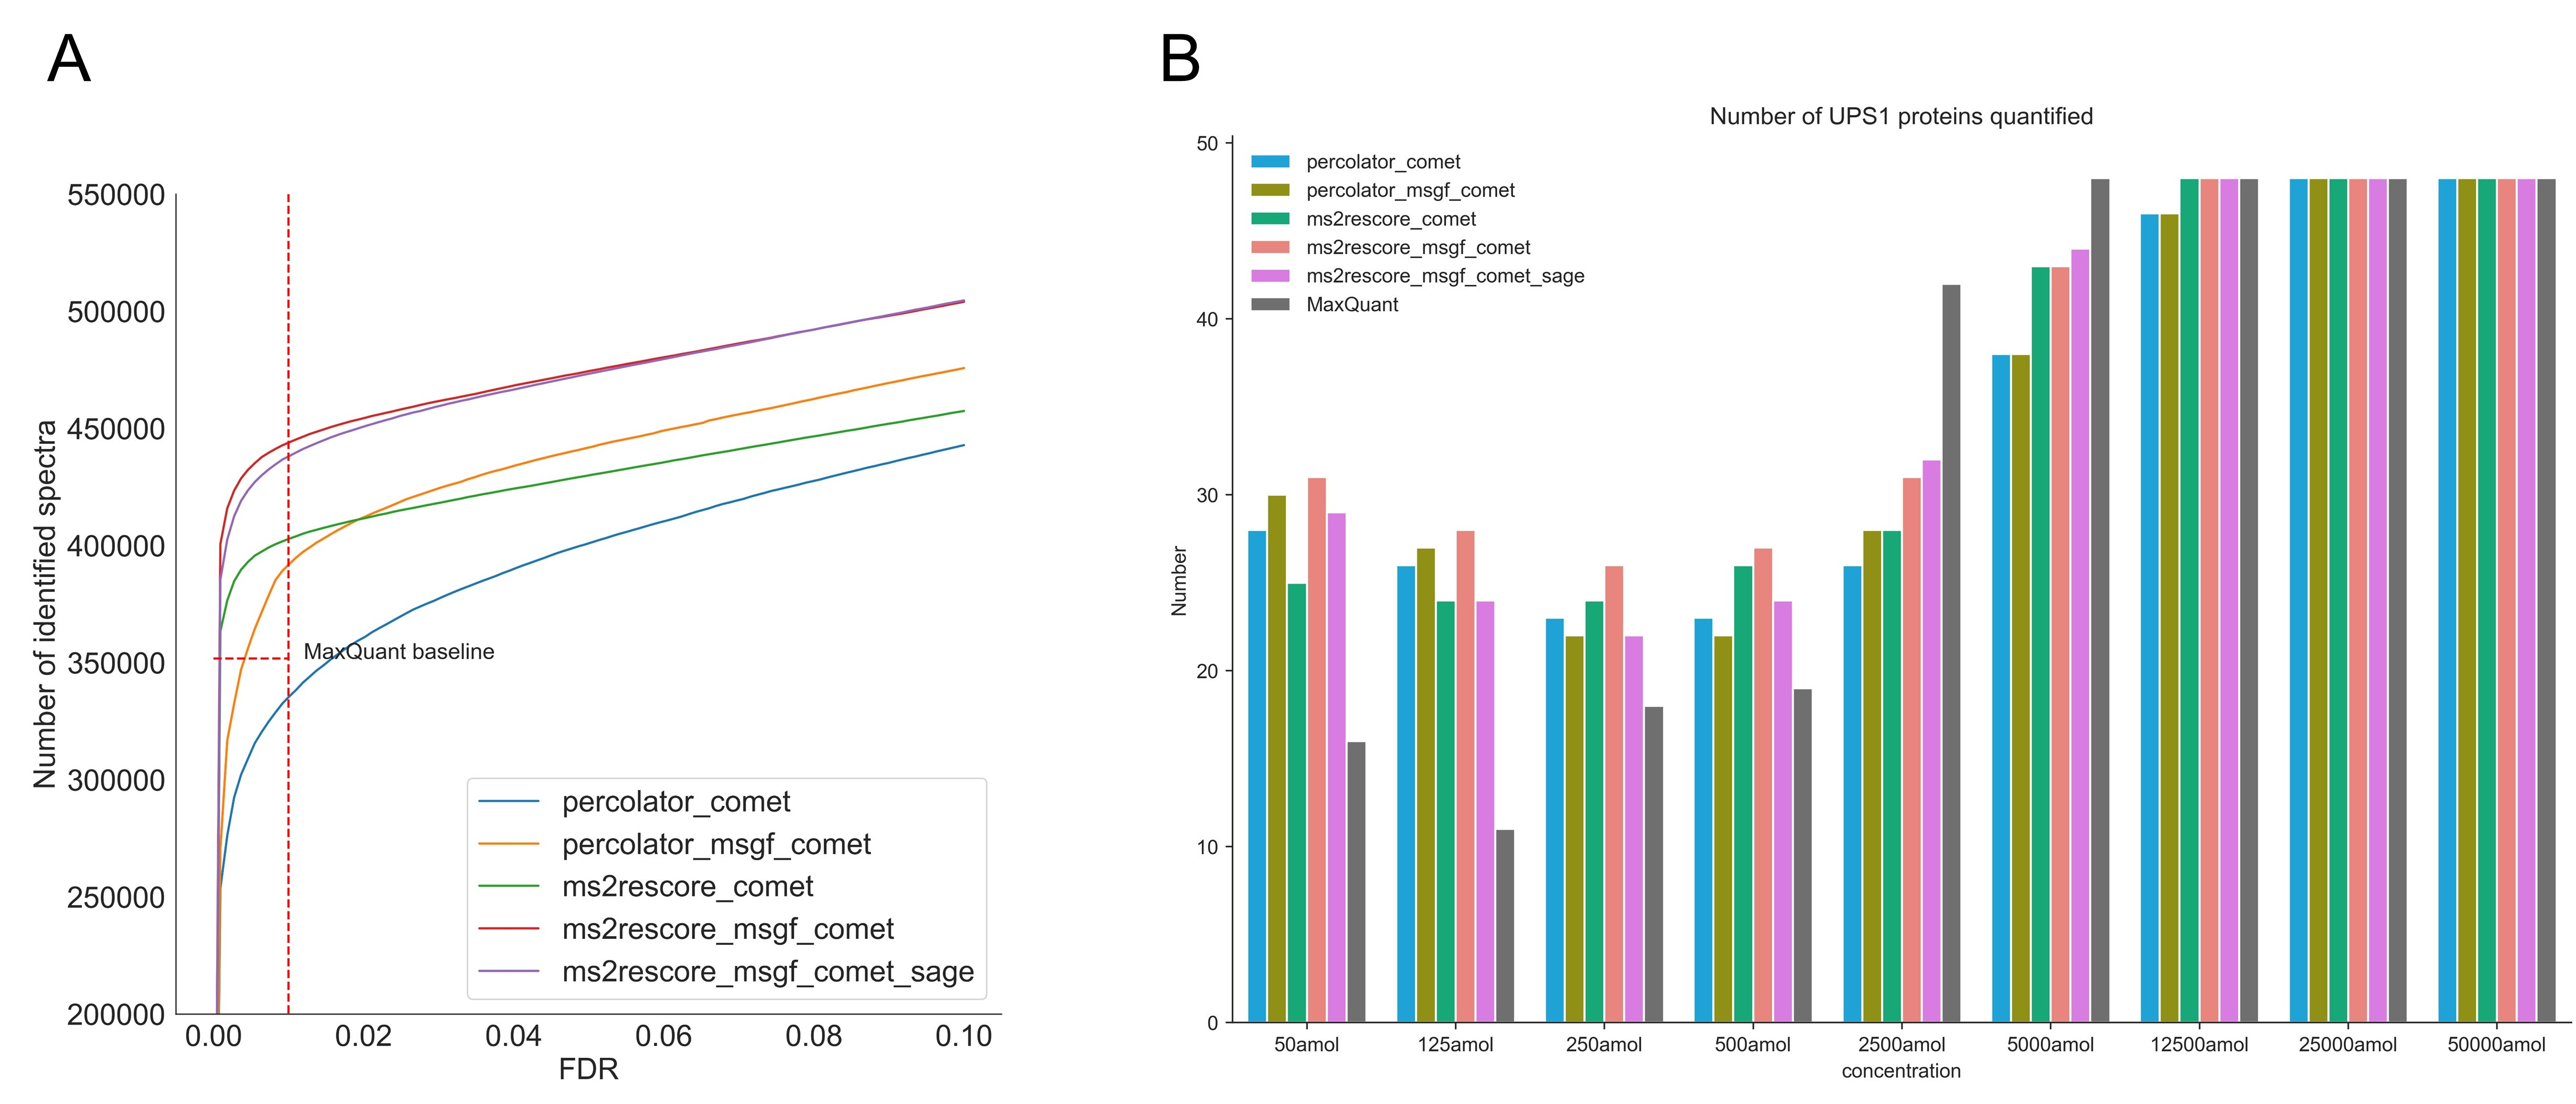
\includegraphics[width=1\textwidth]{figures//PXD001819.jpg}
	\caption{The number of identified spectra as a function of differing FDR levels for different workflow settings. (A) Results for the PXD001819 dataset. (B) Results for the PXD001819 dataset showing protein quantification. Five different workflow settings are shown: the combination of Comet search engine with Percolator rescoring, the combination of Comet with MSGF+, the combination of two search engines with MS2Rescore features, the combination of two search engines with MS2Rescore and SNR features, and the combination of three search engines with MS2Rescore and SNR features. Multiple search engines consensus identification, additional intensity-based and retention time-based features, and SNR features lead to both higher identification rates and high-quality identification.}
	\label{fig:PXD001819_ms2rescore_pic}
\end{figure}

\subsection{quantms integrated with MS2Rescore improves identification and quantification for large-scale TMT experiments}
We then applied this workflow to large-scale TMT experiments from CPTAC. Multiple search engines and rescoring significantly improved peptide identification and protein quantification, as shown in Figure~\ref{fig:PDC_ms2rescore}. The PSM identification rate was improved by 3.6\%, and 921 proteins were newly quantified when DeepLC and MS2PIP features were added, compared to the workflow without MS2Rescore enabled (Figure 2A,B). There are 59 newly quantified proteins whose abundance is located in the top 10\% (Figure 2C). To further explore the impact of these newly quantified proteins from the two search engines with MS2Rescore features workflow on downstream analysis, protein differential expression results from this workflow are shown in Figure 2. There are 27 newly quantified proteins that are significantly differentially expressed (Figure 2D). Among them, Yang et al. reported an association between significant upregulation of FOXG1 protein and prognosis in Clear Cell Renal Cell Carcinoma [10.18632/aging.204448]. This further illustrates that by incorporating rescoring features based on MS2PIP and DeepLC, the approach not only improves the sensitivity of spectral identification but also facilitates protein quantification, which ultimately contributes to biological knowledge discovery.

Moreover, we extracted the top 20 SVM weights from Percolator to explore the impact of different features on rescoring for different search engines, shown in Supplemental Figure~\ref{fig:PDC_ms2rescore_weights}. For Comet identification results, SpecPearsonNorm, DotProdIonYNorm, and RtDiffBest features have significant weights for final rescoring. The weight of SpecPearsonNorm is positive, indicating that a high SpecPearsonNorm value between MS2PIP prediction and experimental intensities corresponds to a better hit. The weight of RtDiffBest is negative, indicating that large differences between observed and calculated retention time correspond to a worse score. It is interesting that peptide length becomes a significant feature after adding MS2Rescore features. The positive value demonstrates higher scores for longer peptides. One potential explanation for this phenomenon is that short peptides are less conducive to search engine identification due to fewer fragment ions. For the other two search engines, similar distributions of weights can be observed. SpecPearsonNorm, DotProdIonYNorm, and RtDiffBest features still have significant weights.

% Figure Example
\begin{figure}[ht!]
	\centering
	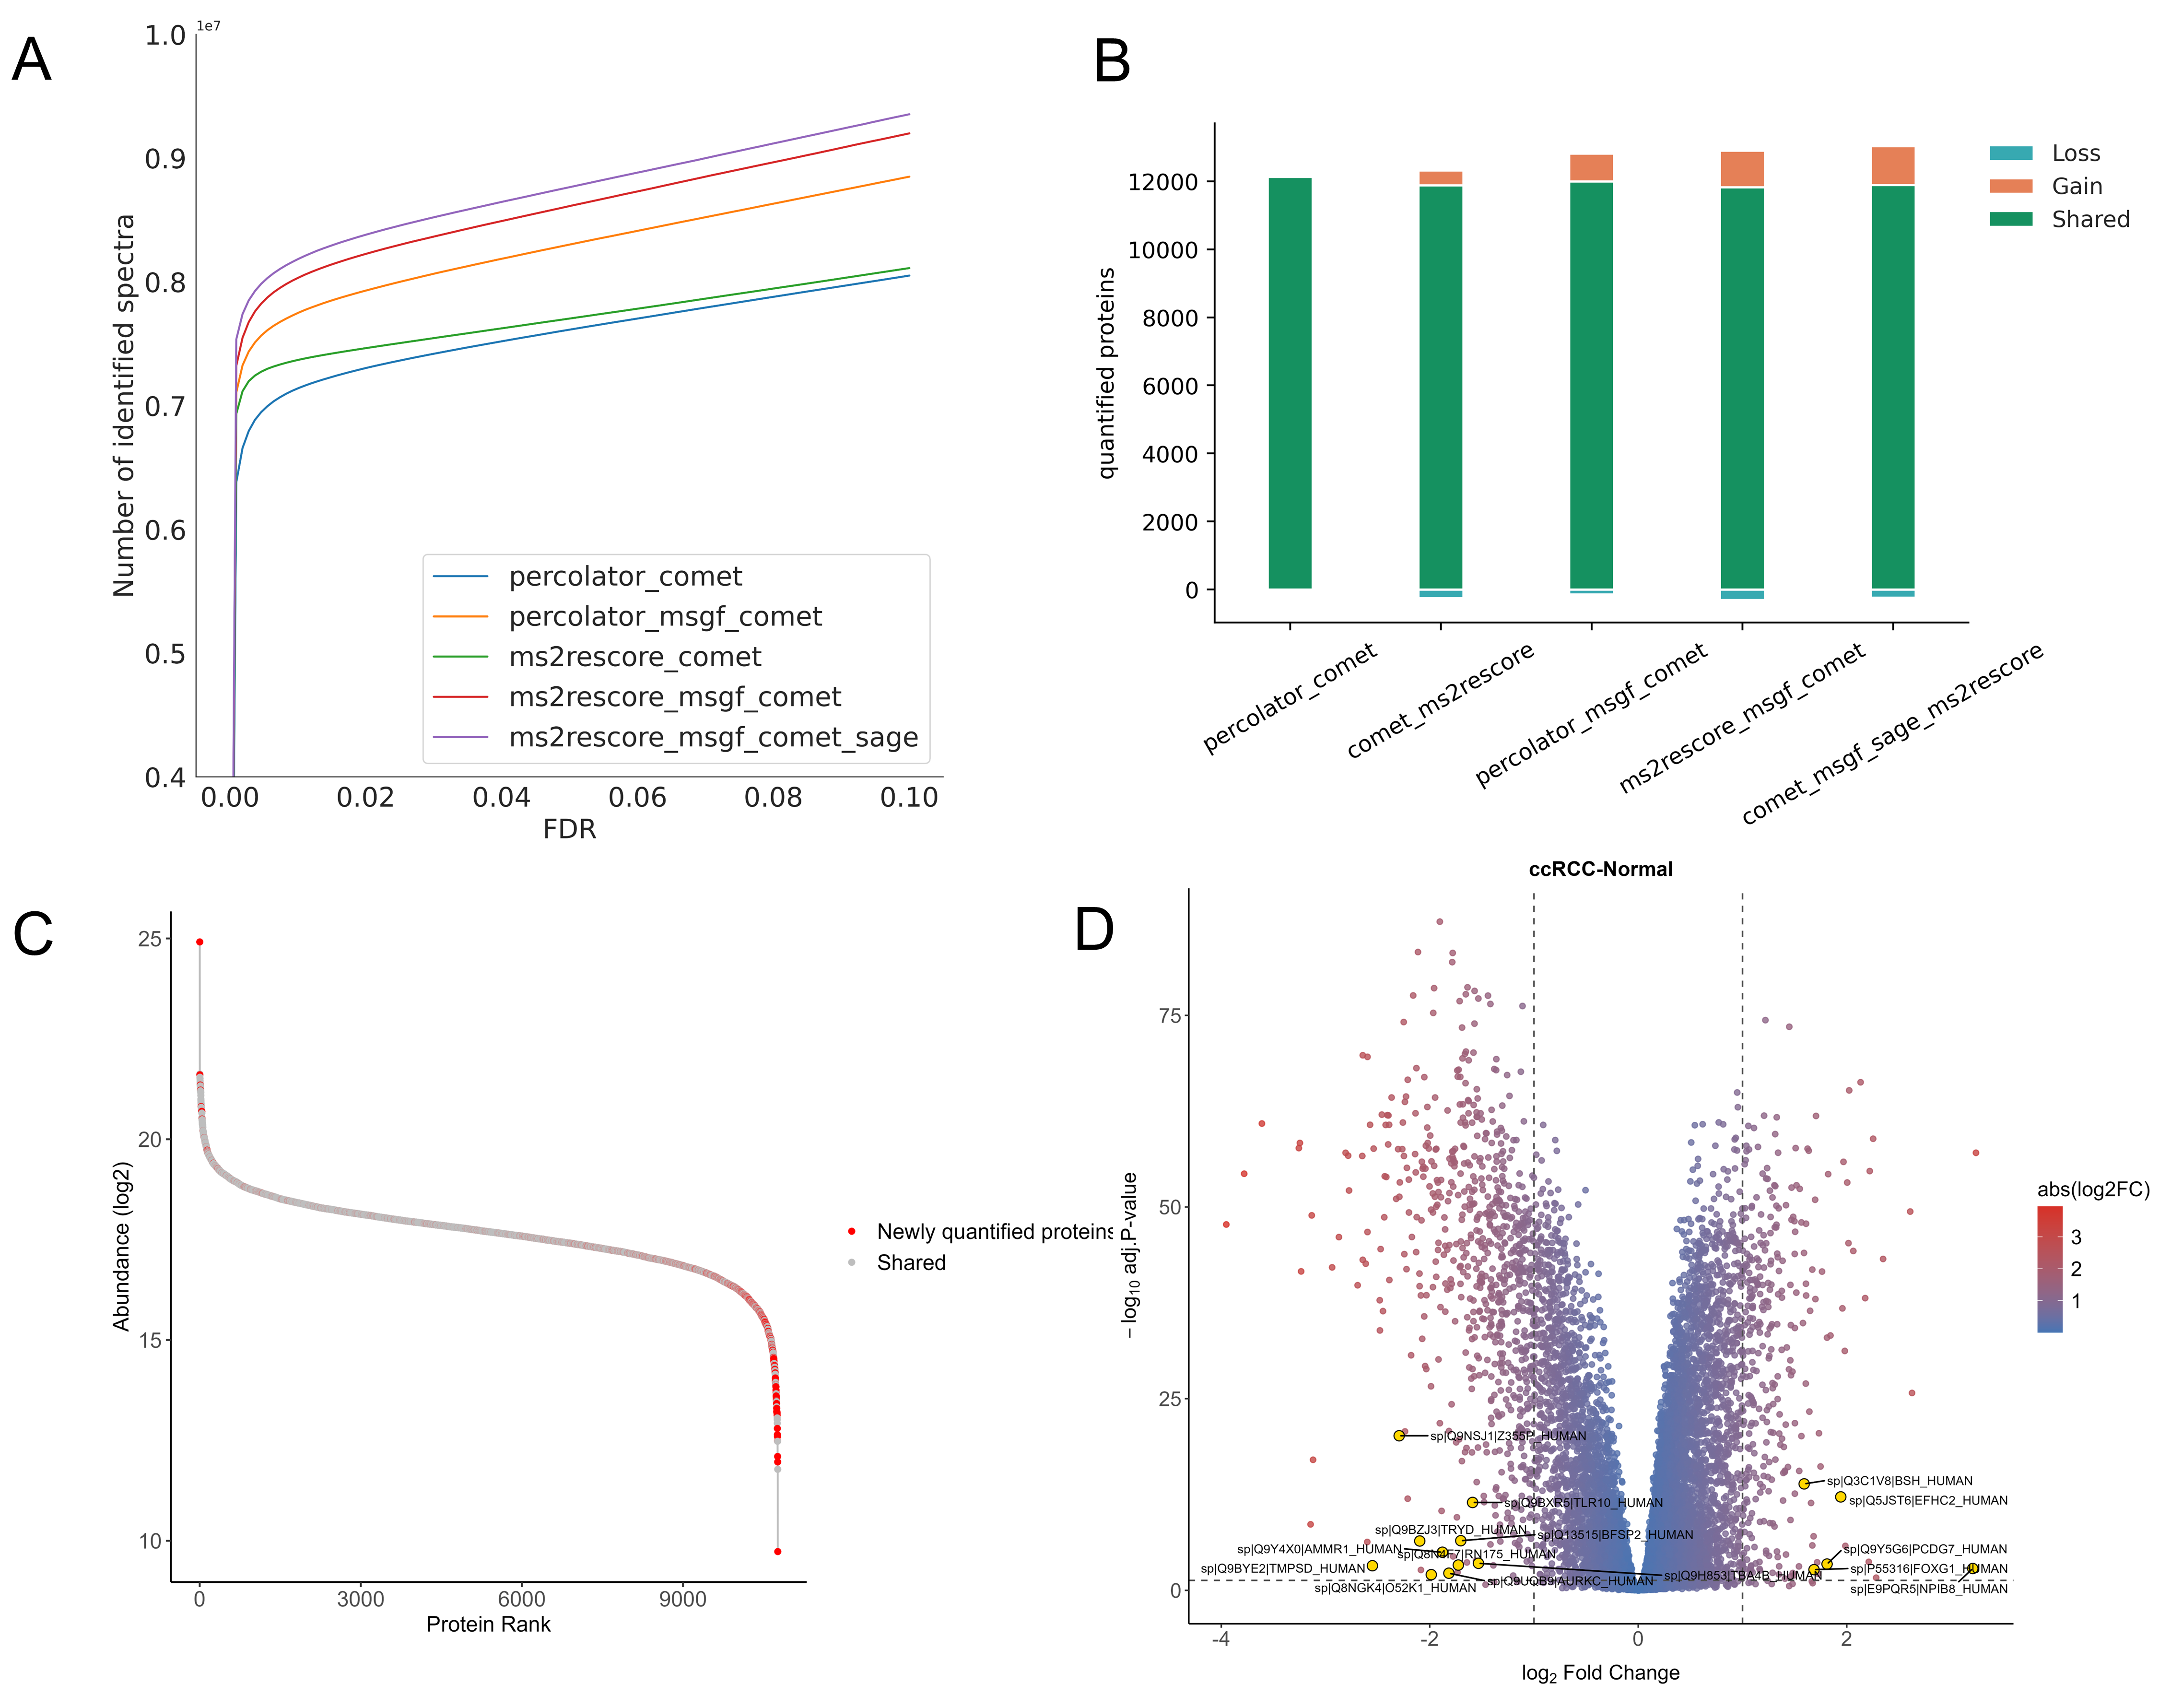
\includegraphics[width=1\textwidth]{figures//CPTAC_TMT.png}
	\caption{Comparison of identification and quantification results for different workflow settings. (A) The number of identified spectra as a function of differing FDR levels for different workflow settings. (B) The number of quantified proteins. The green part indicates the intersection between a workflow and Comet results. (C) The rank of protein abundance from Comet and MSGF+ with MS2Rescore. The red dots represent proteins quantified only in the Comet and MSGF+ with MS2Rescore workflow compared to the Comet and MSGF+ workflow without MS2Rescore. (D) The volcano plot for differential expression analysis from MSstatsTMT. The red dots represent proteins quantified only in the Comet and MSGF+ with MS2Rescore workflow compared to the Comet and MSGF+ workflow without MS2Rescore.}
	\label{fig:PDC_ms2rescore}
\end{figure}

\subsection{Evaluation of quantms integrated with MS2Rescore on HLA Class I Peptides}
Furthermore, we evaluated the performance of the quantms identification workflow on the immunopeptides dataset PXD019643. Therefore, four different workflow settings were compared: the combination of Comet search engine with Percolator rescoring, the combination of Comet with MSGF+, the combination of two search engines with MS2Rescore features, and the combination of two search engines with MS2Rescore and SNR features. These were compared in terms of the total amount of identifications as well as the number of unique identifications based on sequence. Overall, multiple search engines and rescoring with MS2Rescore substantially improved the spectrum identification rate compared to using only the Comet search engine or no rescoring at both 1\% and 0.1\% FDR. Multiple search engines achieved an 11.7\% increase in the number of identified spectra compared to using only Comet search engines, and MS2Rescore features further increased the number of identified spectra by 22.8\% compared to multiple search engines without MS2Rescore features, as shown in Figure~\ref{fig:PXD019643_immunopeptides}.

The power of providing these predictions to Percolator is further illustrated when visualizing the distributions for decoy PSMs, rejected target PSMs, and accepted target PSMs from individual support and consensus supports (Figure 3C, D). The accepted target PSMs are clearly separable from the decoy and rejected target PSMs using only the Pearson correlation coefficient (PCC). The distributions for accepted targets from individual support and consensus supports are highly similar in that they both exhibit low retention time errors and high PCC values. This further demonstrates that quantms is effective for integrating the identification scores of multiple search engines.

% Figure Example
\begin{figure}[ht!]
	\centering
	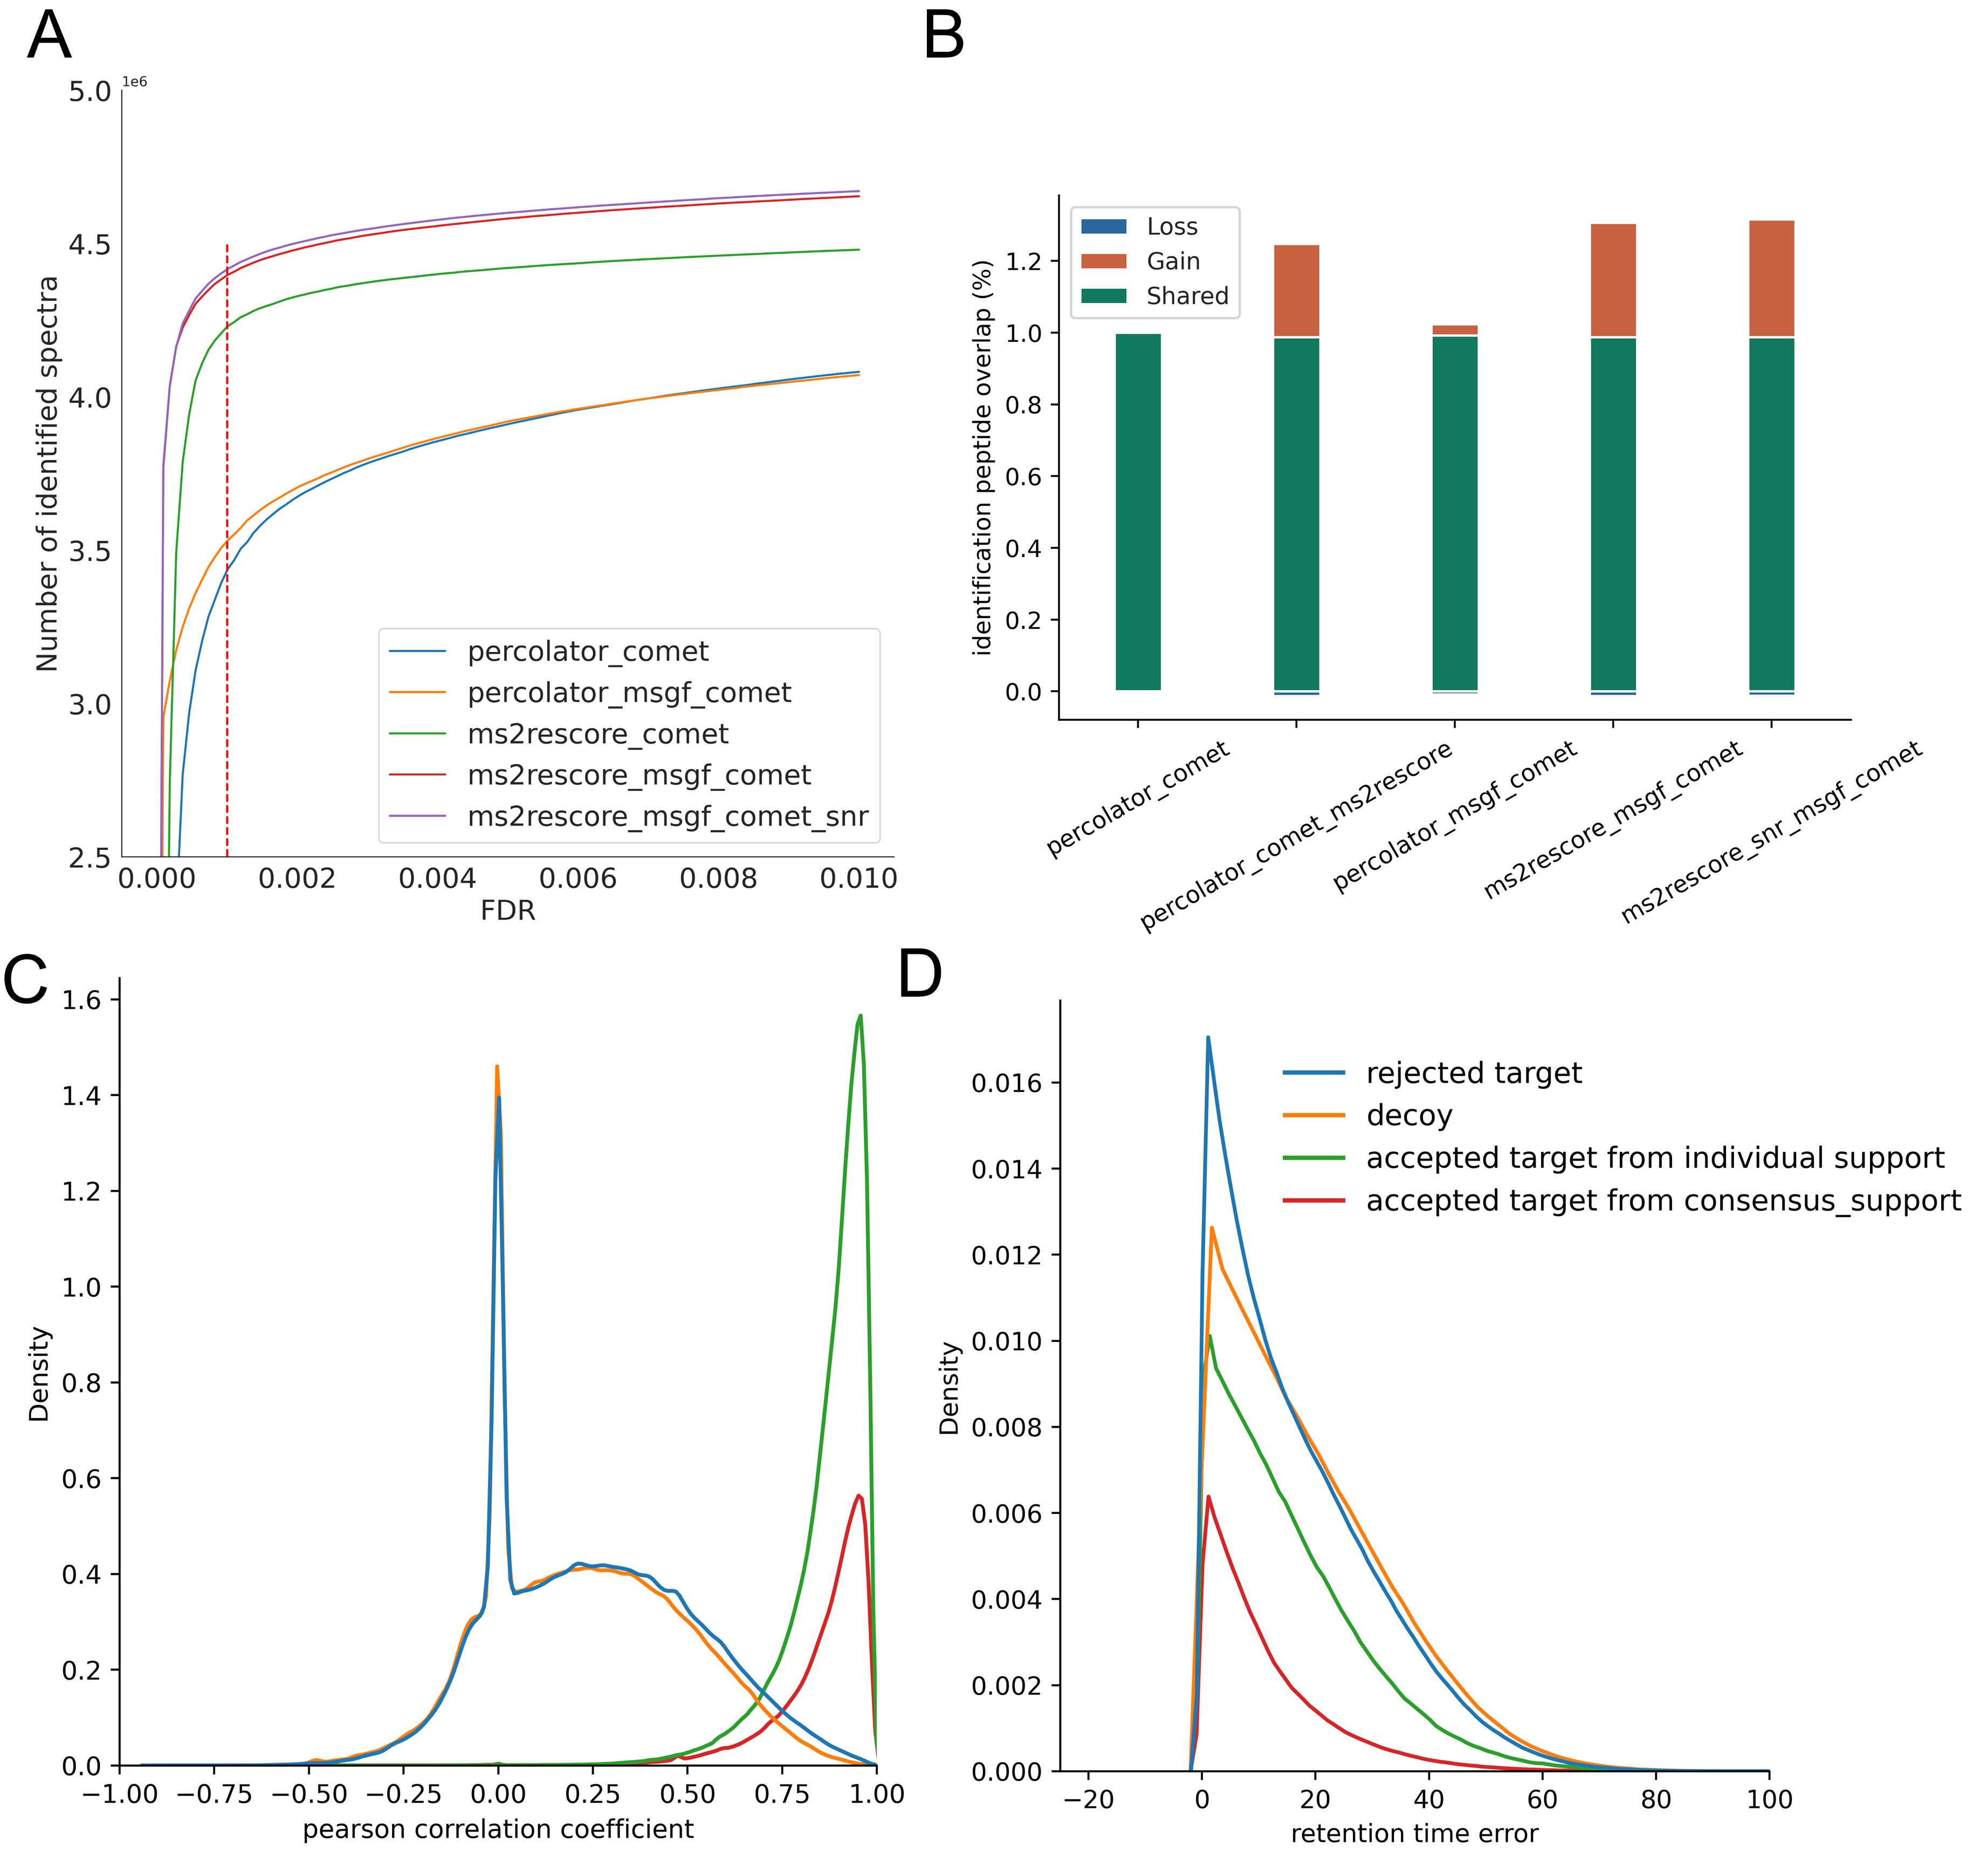
\includegraphics[width=1\textwidth]{figures//PXD019643.png}
	\caption{Comparison of immunopeptides identification results for different workflow settings. (A) Line plot showing the number of spectra identified for four workflow settings at different PSM FDR levels. (B) Percentage of unique identified peptides using different workflow settings. Density plots showing the distribution of the smallest retention time error between observed and predicted retention time (C) and the Pearson correlation between observed and predicted peak intensities (D) for each PSM split into decoys (red), rejected targets with q-value $>$0.01 (blue), and accepted targets from individual support and consensus support with q-value $<$0.01 (green). Note that the rejected targets distribution coincides with the decoy distribution.}
	\label{fig:PXD019643_immunopeptides}
\end{figure}

\subsection{quantms integrated with MS2Rescore facilitates the identification of phosphorylated peptides}
In addition, we investigated the performance of our quantms workflow with MS2Rescore on post-translational modification experiments (PXD026824). For phosphoproteomics analyses, different workflow settings were evaluated: (1) Comet alone, (2) Comet combined with MSGF+, and (3) multiple search engines combined with MS2Rescore features. These were processed using Percolator to determine whether multiple search engines and MS2Rescore facilitated the identification and quantification process. In Figure~\ref{fig:PXD026824_ms2rescore}, it is clearly visible that the introduction of multiple search engines consensus identification and MS2Rescore features extensively improves the stringency with which Percolator can classify PSMs. This is illustrated by the remarkable shift to the left compared with Comet alone. In addition, there is also a gain in identification rate, which is shown in the vertical direction of this figure. The two search engines consensus identification combined with MS2Rescore features enabled a 19\% increase in the number of identified spectra compared to consensus identification without MS2Rescore (Figure 4A). The top 20 weights from Percolator are shown in Supplemental Figure~\ref{fig:phospho_features}. We can observe the same features as in the above results, such as the DotProdIonYNorm feature.

Protein phosphosite false localization rate (FLR) control is necessary for phosphoproteomics analysis. Therefore, we also investigated the effect of different workflow settings on phosphorylated peptides at different FLR levels (Figure 4B, C). The search engines consensus identification combined with MS2Rescore features increased the number of phosphorylated peptide identifications by 17\% at 0.01 local FLR compared to the approach without MS2Rescore. There are 1,345 phosphorylated peptides quantified only in the consensus identification combined with MS2Rescore process. Considering protein phosphosites, consensus identification combined with the MS2Rescore process newly reports 350 protein phosphorylation sites (Figure 4D). Altogether, these results show that quantms integrated with MS2Rescore can boost performance in phosphoproteomics.

% Figure Example
\begin{figure}[ht!]
	\centering
	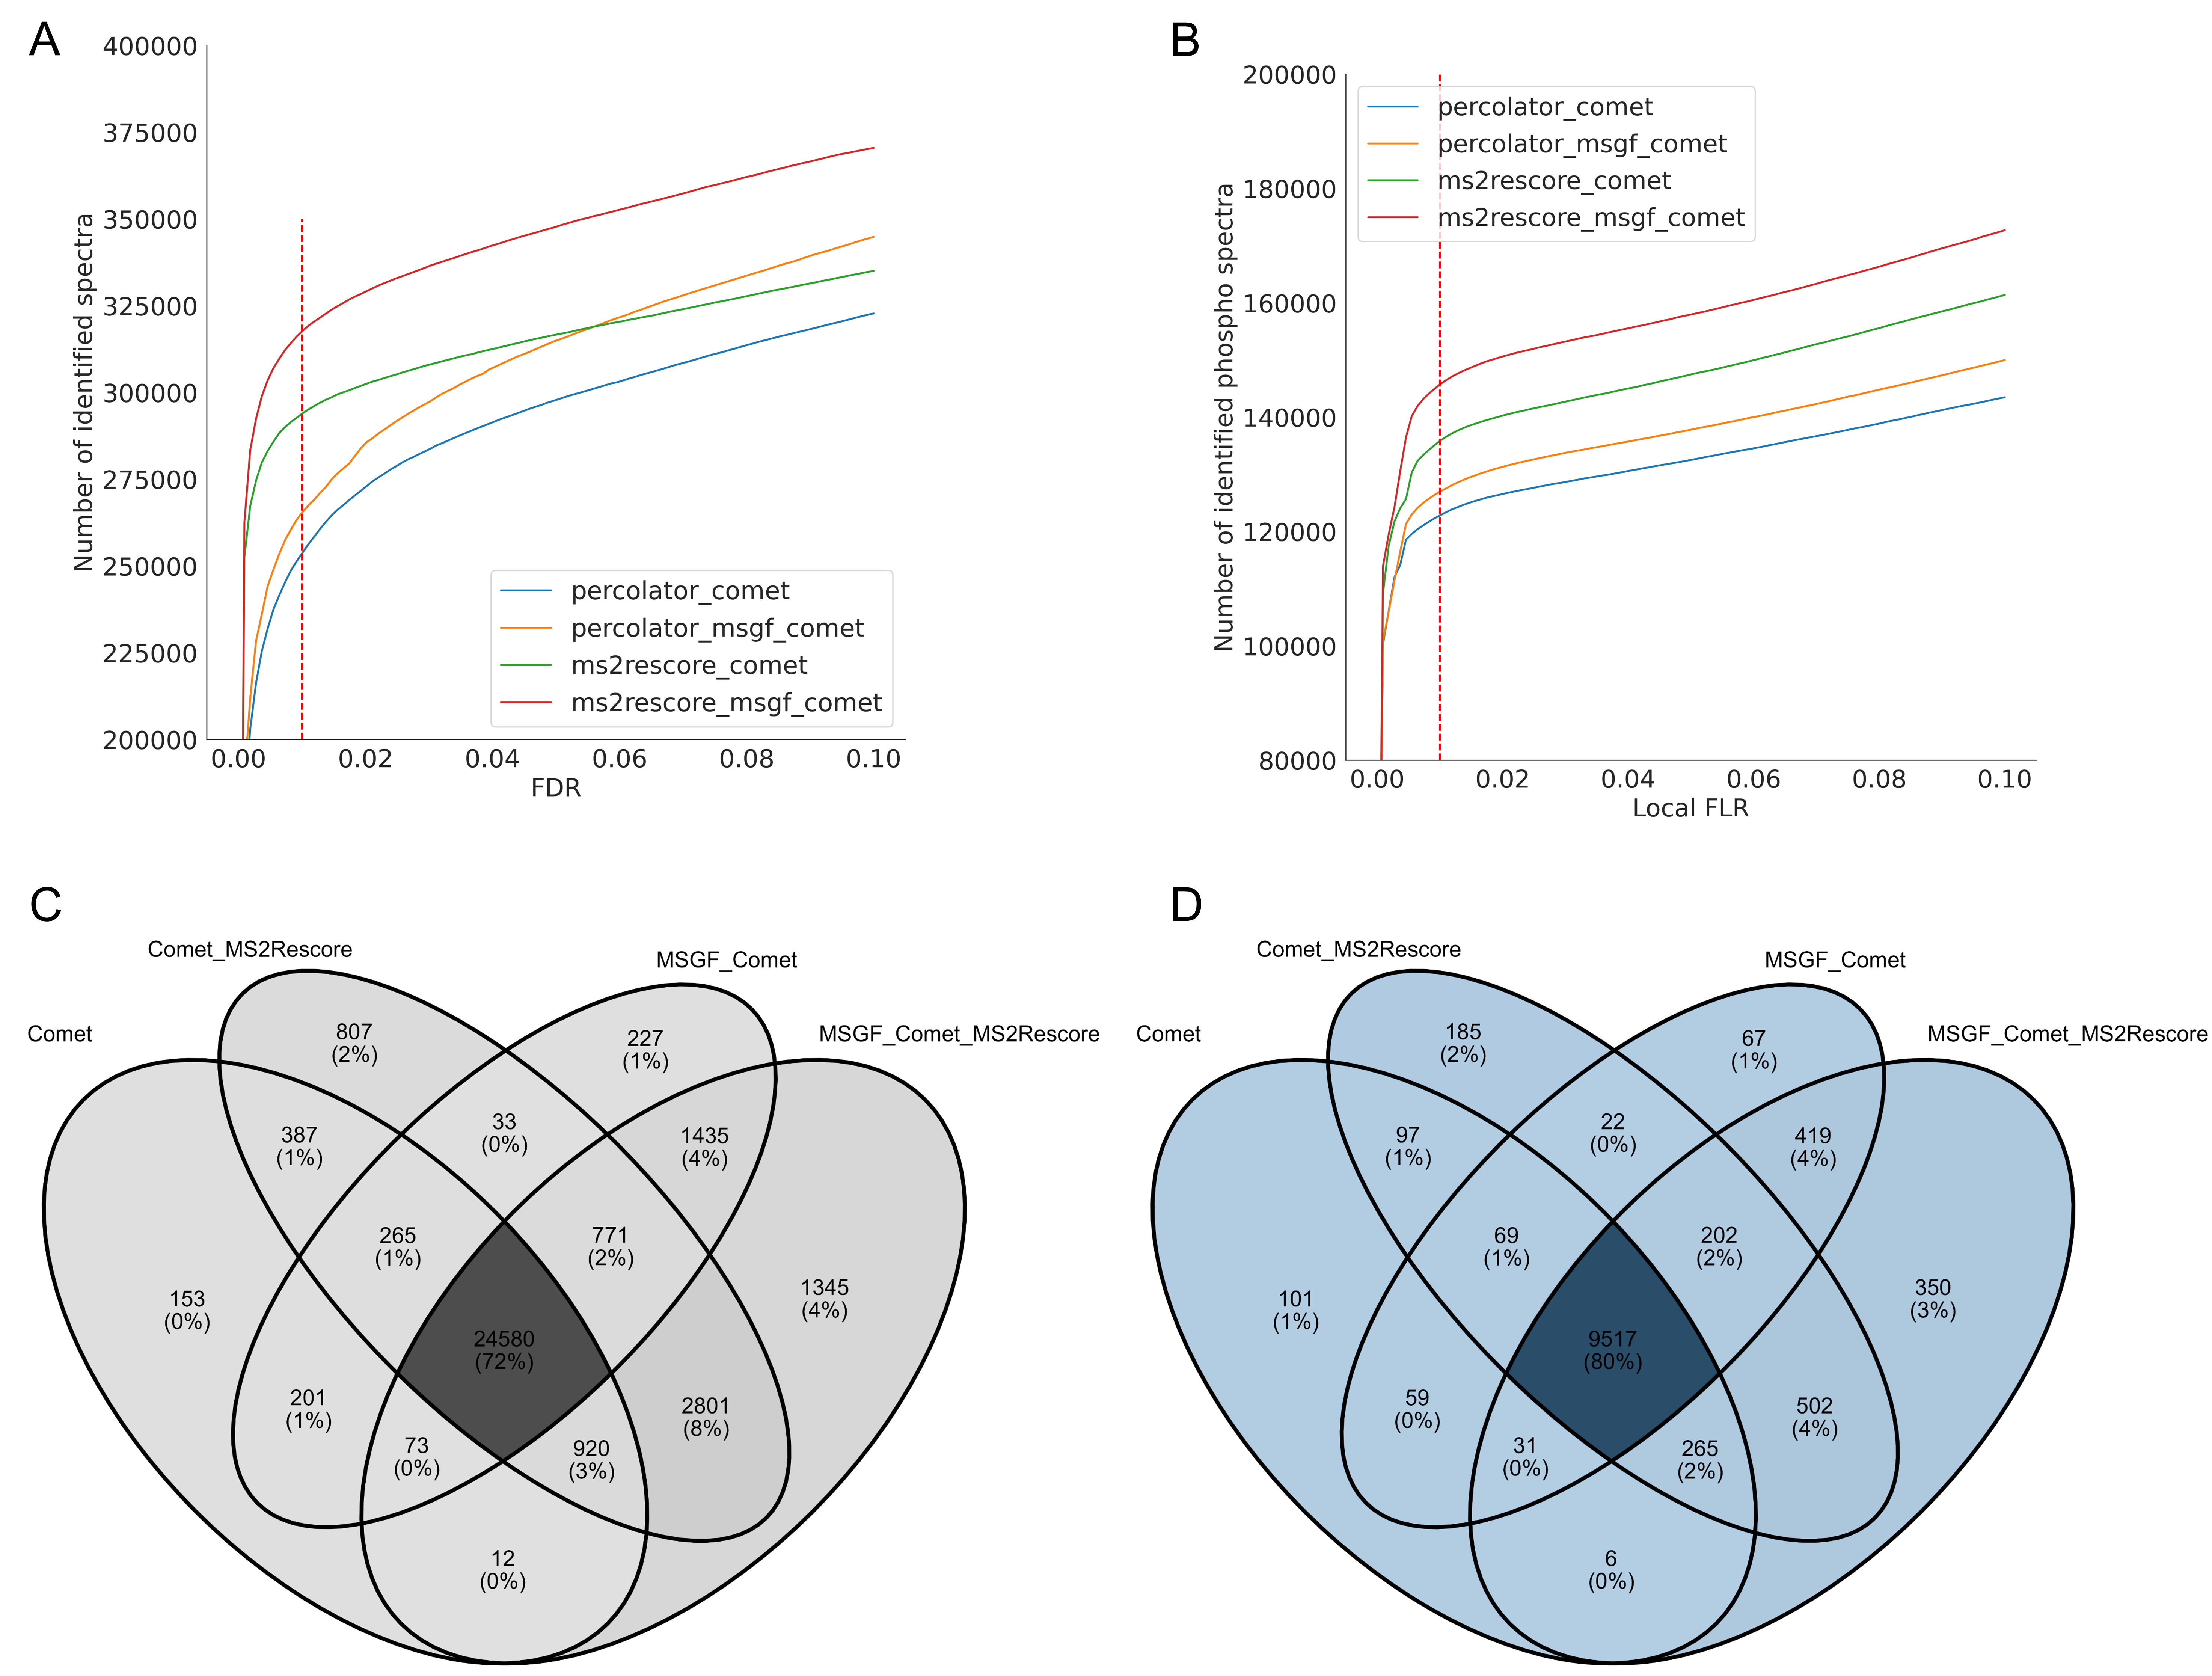
\includegraphics[width=1\textwidth]{figures//phospho2.png}
	\caption{Comparison of phosphorylated peptide identification results for different workflow settings. (A) Line plot showing the number of spectra identified for four workflow settings at different PSM FDR levels. (B) Line plot showing the number of phosphorylated spectra identified for four workflow settings at different local false localization rate levels after an FDR of less than 0.01 at the PSM level. (C) Venn diagram of peptides quantified for four settings. (D) Venn diagram of protein phosphosites at protein FDR 0.01 and FLR 0.01 for four settings.}
	\label{fig:PXD026824_ms2rescore}
\end{figure}

\section{Discussion}
Advancements in deep learning-based tools have significantly improved the accuracy and sensitivity of peptide-spectrum match (PSM) rescoring, yet their integration into streamlined, reproducible, and quantitative proteomics workflows has remained limited, especially for large-scale public data analysis. In this study, we demonstrate the systematic incorporation of MS2Rescore into the open-source quantms pipeline and evaluate its impact across various experimental settings, including label-free quantification (LFQ), tandem mass tag (TMT)-based quantification, immunopeptidomics, and phosphoproteomics. Our results show that enhanced feature sets derived from MS2PIP and DeepLC not only improve identification rates but also translate into gains in quantification depth. Importantly, we provide evidence that the improved identifications via rescoring propagate downstream into quantification, leading to increased numbers of proteins with reliable abundance estimates, as well as enhanced detection of differentially expressed proteins.

To demonstrate the applicability and advantages of quantms integrated with MS2Rescore in quantitative proteomics, we performed a series of reanalyses using publicly available large-scale datasets with well-established benchmarks. In label-free experiments, MS2Rescore-enhanced workflows achieved significant increases in PSM and peptide identification while maintaining or improving quantification reproducibility across replicates. For TMT experiments, the integration of MS2Rescore into quantms increased the number of quantifiable proteins. In more challenging applications, such as immunopeptidomics and phosphoproteomics, the deep learning-based rescoring pipeline consistently yielded higher identification rates and improved sensitivity. These improvements contribute meaningful biological insights, such as phosphosite discovery and the identification of differentially expressed proteins with potential clinical relevance.

Overall, the results in this publication highlight the synergistic benefits of integrating machine learning-based features within end-to-end, cloud-based proteomics workflows. By embedding MS2Rescore into the quantms pipeline, we provide a practical and accessible solution for the community to leverage cutting-edge spectral prediction and retention time modeling without the need for complex manual configuration. This integrated approach enables reproducible reanalysis of large public datasets, increases identification confidence, and strengthens quantitative conclusions across diverse experimental designs. Future work will focus on expanding this approach to other types of post-translational modifications and exploring the integration of additional machine learning tools to further enhance proteomics data analysis capabilities.

\section*{Acknowledgments}
We thank all those who supported this research, including funding bodies and the proteomics community for making public datasets available. 
Yasset Perez-Riverol would like to acknowledge funding from EMBL core funding, Wellcome grants (208391/Z/17/Z, 223745/Z/21/Z) and the BBSRC grant ‘DIA-Exchange’ [BB/X001911/1].

% References Section
\bibliographystyle{unsrt}  % Unsorted style for natbib
\bibliography{references}  % references.bib file contains your bibliography

\renewcommand\thefigure{S\arabic{figure}}
\setcounter{figure}{0}

% Figure Example
\begin{figure}[ht!]
	\centering
	\includegraphics[width=1\textwidth]{figures//LFQ_weights.png}
	\caption{The weights that Percolator assigns to different features of the search engine feature vector in MSGF+ (A), Comet (B), and SAGE (C) combined with Percolator settings from PXD001819. The more different from zero a weight is (both positive and negative), the more important that feature is in the final Percolator classification.}
	\label{fig:PXD001819_svm_weights}
\end{figure}

% Figure Example
\begin{figure}[ht!]
	\centering
	\includegraphics[width=1\textwidth]{figures//CPTAC_weights.png}
	\caption{The top 20 normalized weights from Percolator for MSGF+ (A), Comet (B), and SAGE (C) identification results from PDC000125.}
	\label{fig:PDC_ms2rescore_weights}
\end{figure}

\begin{figure}[ht!]
	\centering
	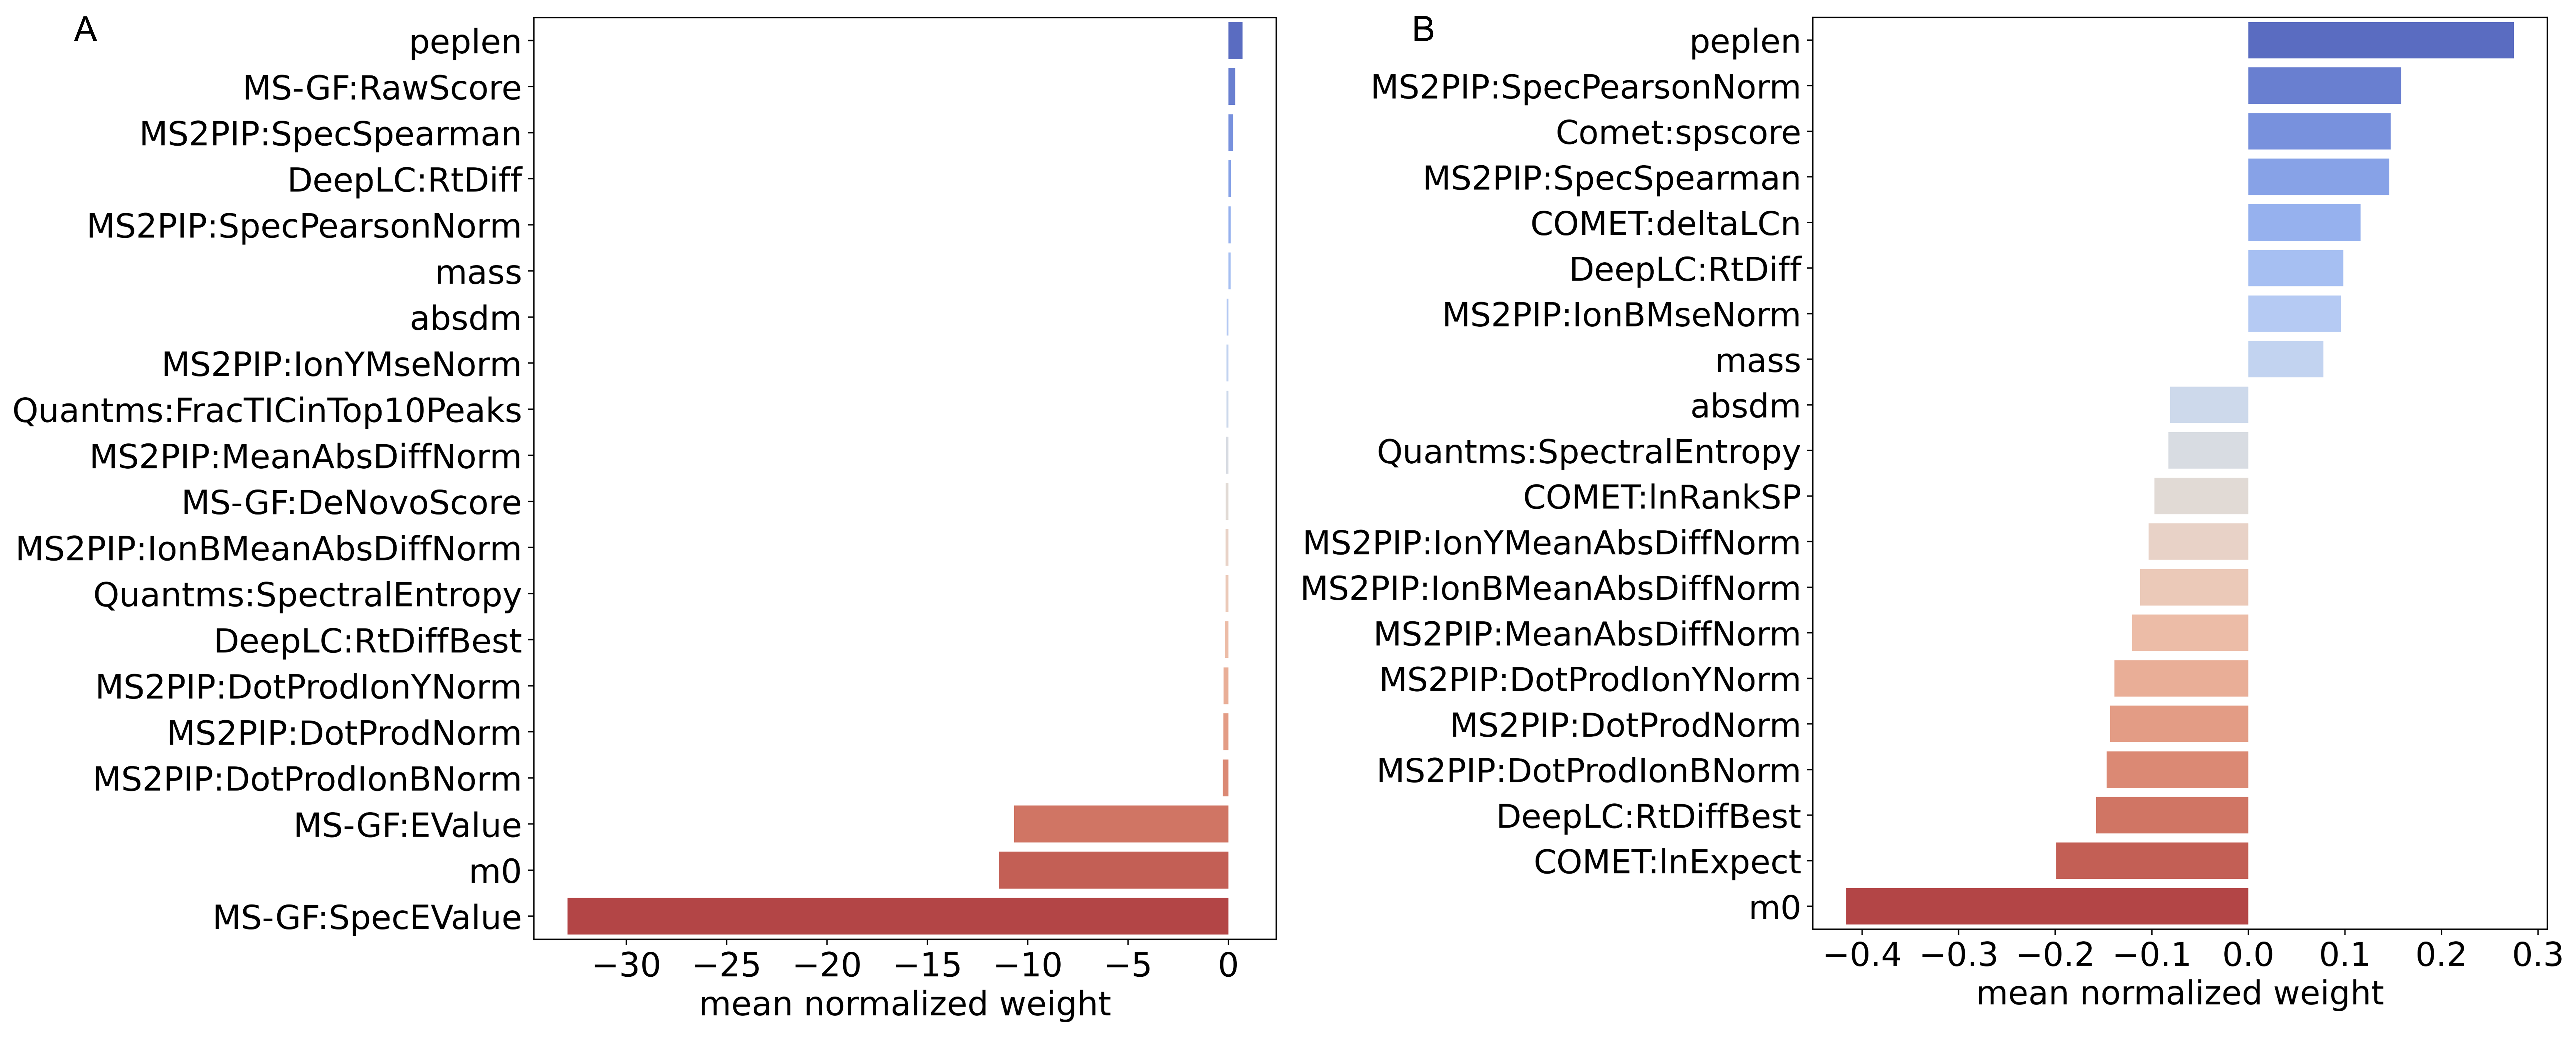
\includegraphics[width=1\textwidth]{figures//PXD019643_weights.png}
	\caption{The top 20 normalized weights from Percolator for MSGF+ (A) and Comet (B) identification results in the PXD019643 dataset.}
	\label{fig:PXD019643_features}
\end{figure}

\begin{figure}[ht!]
	\centering
	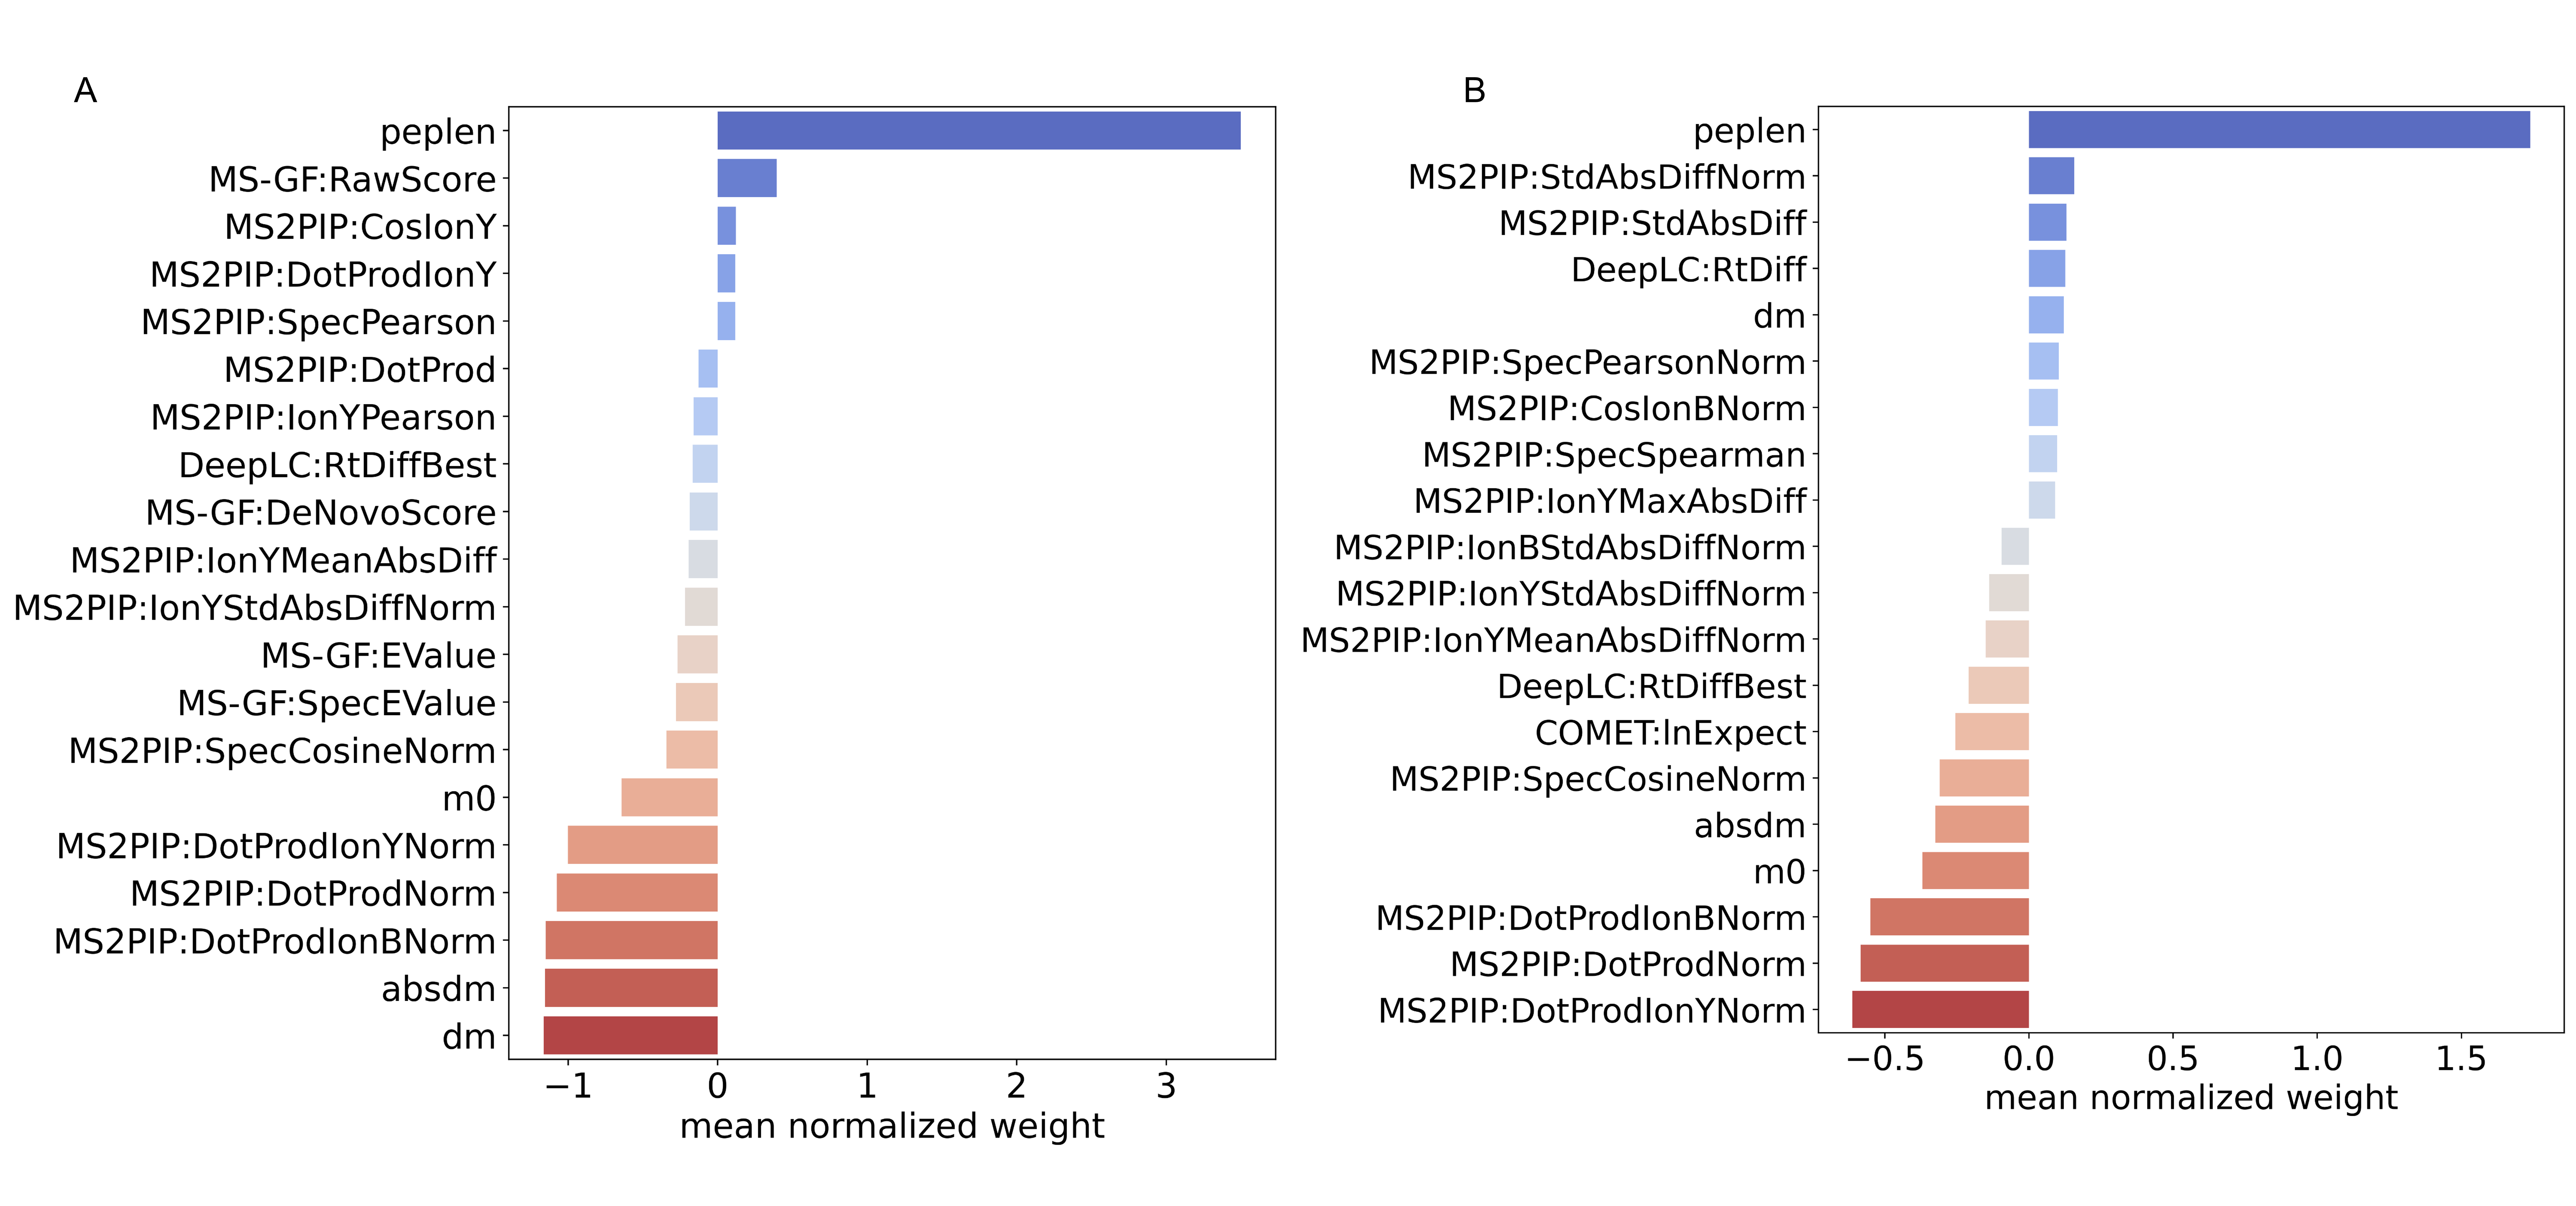
\includegraphics[width=1\textwidth]{figures//phos_weights.png}
	\caption{The top 20 normalized weights from Percolator for MSGF+ (A) and Comet (B) identification results in the PXD026824 dataset.}
	\label{fig:phospho_features}
\end{figure}

\end{document}

